\documentclass[../bericht.tex]{subfiles}

\begin{document}

  \begin{appendices}

    \section{Netzteil-Kennlinie}
    \label{sec:netzteil-kennlinie}
      \Cref{fig:netzteil-kennlinie} zeigt die für die Berechnung der Laserschwelle in \cref{subsec:laserschwelle} verwendete Charakterisitk des verwendeten Netzteils.

      \begin{figure}[H]
        \centering
        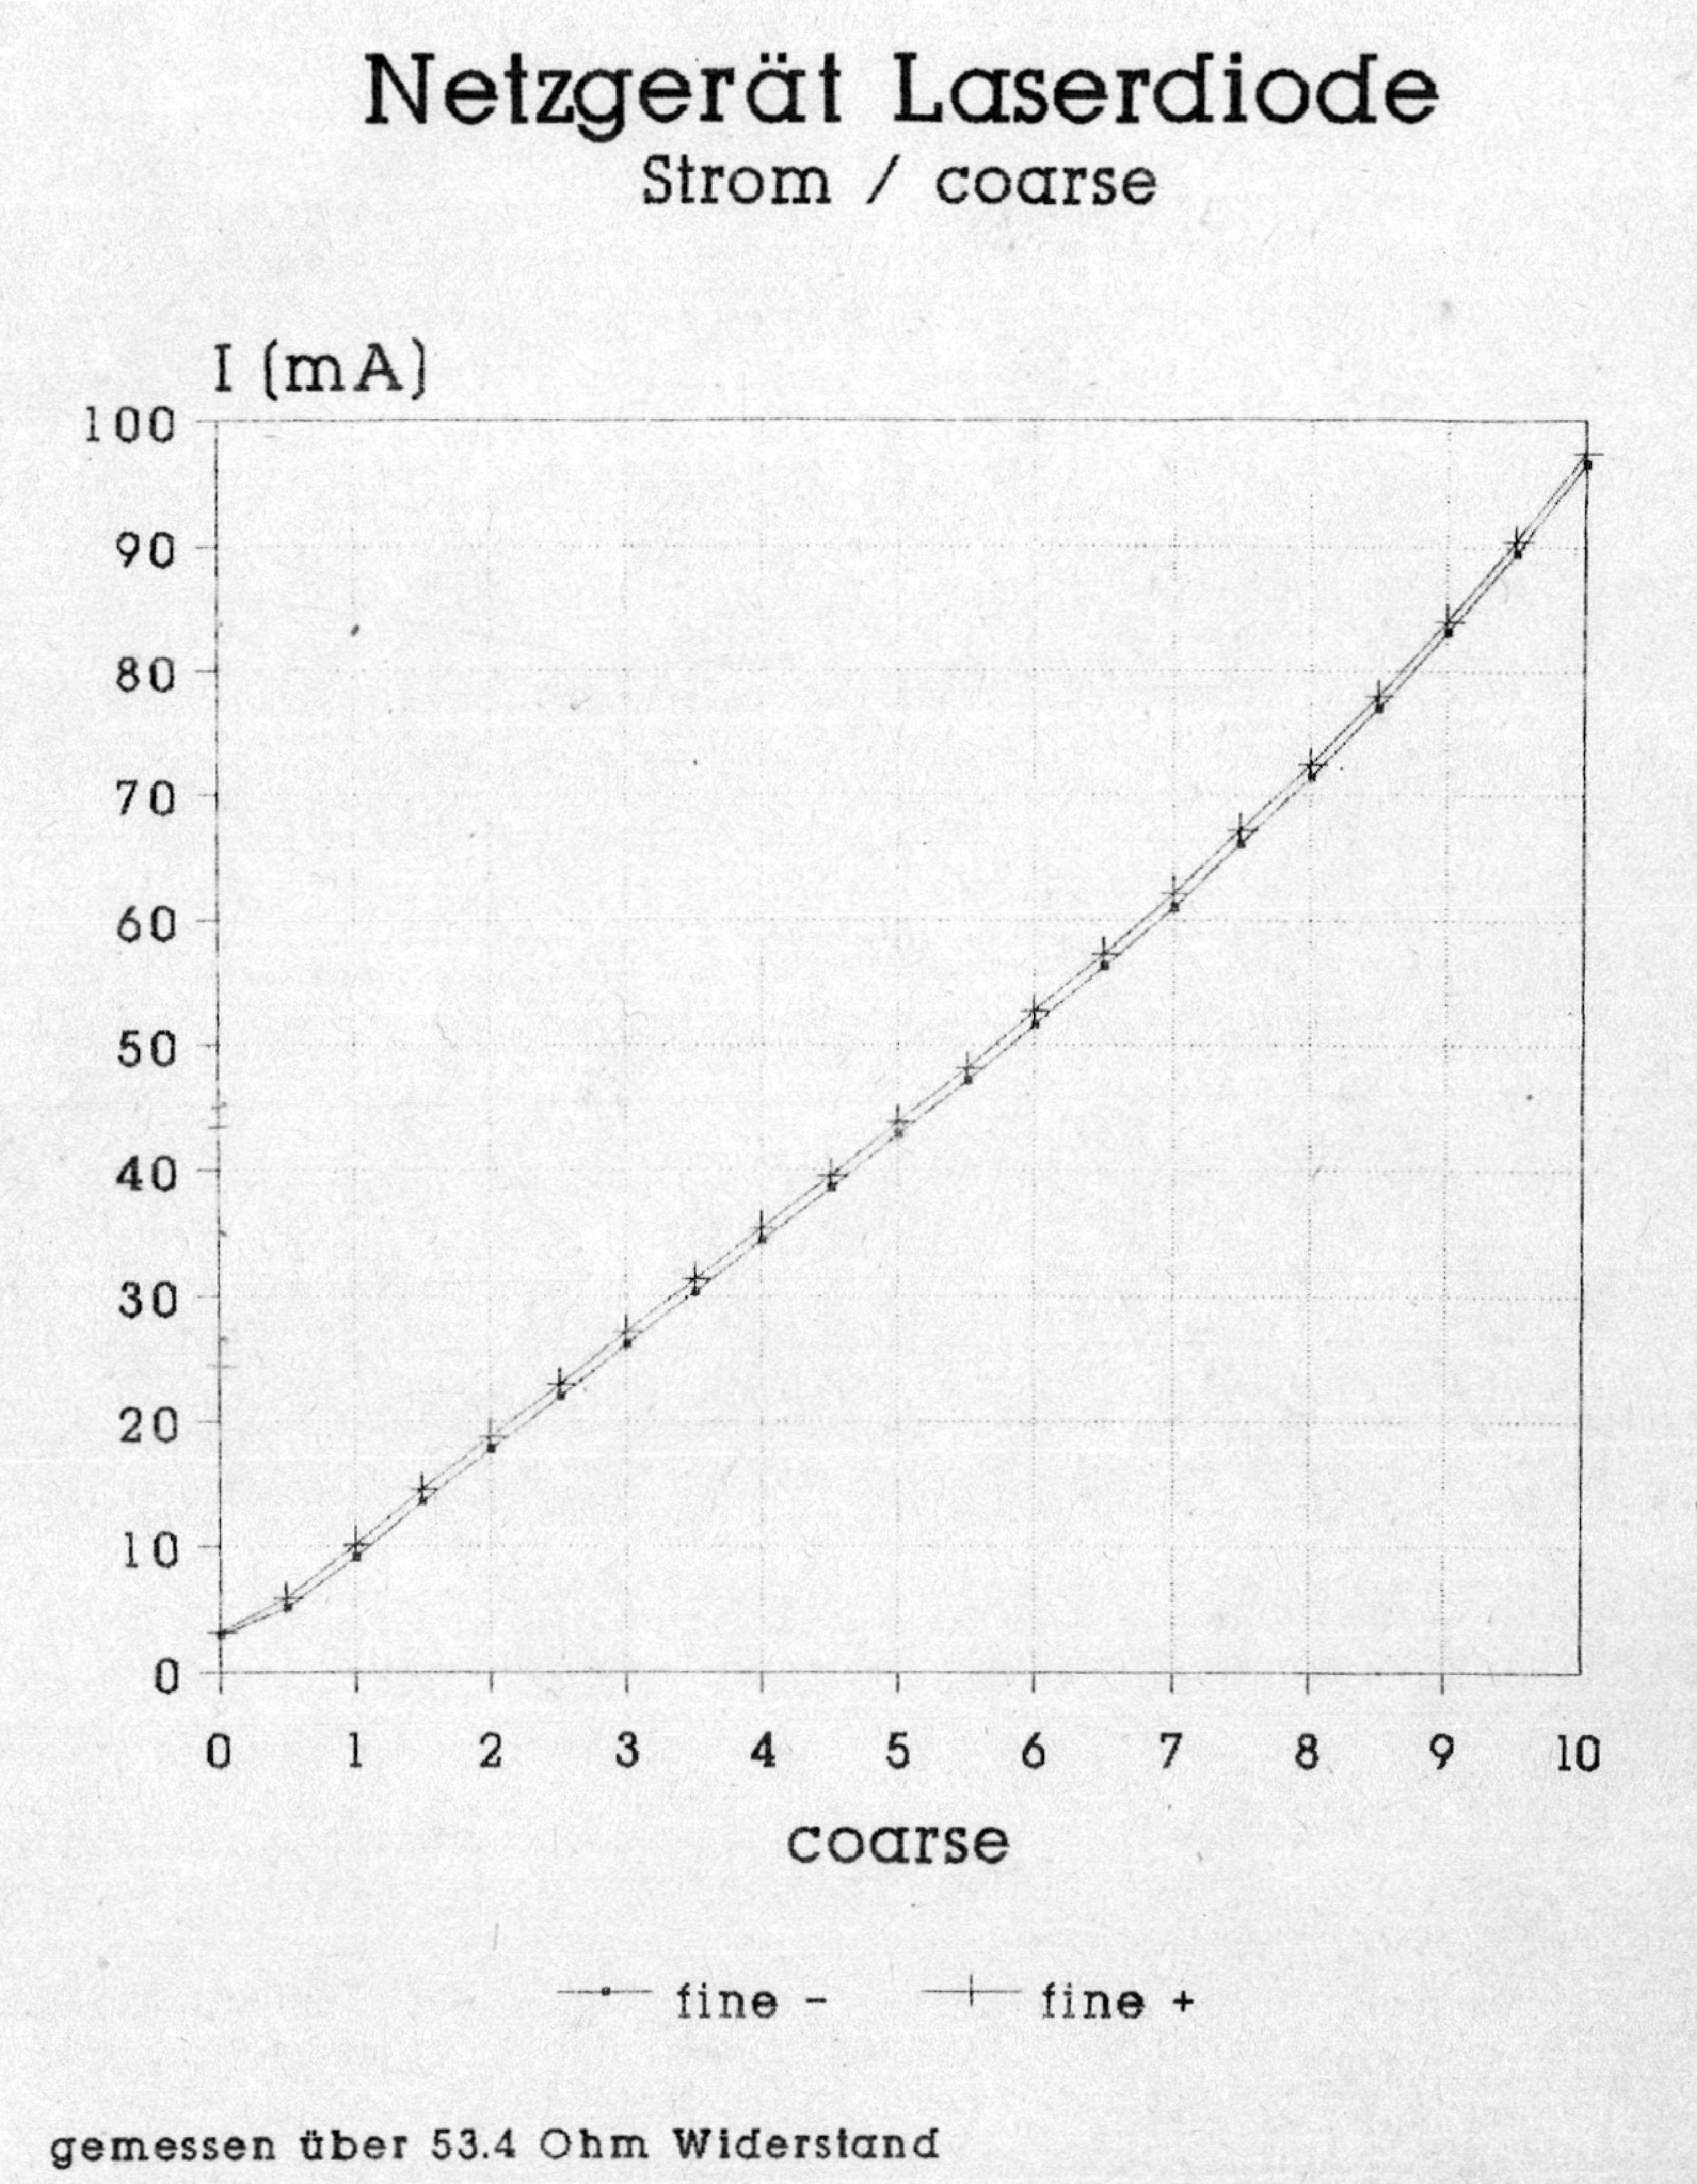
\includegraphics[width=0.85\textwidth]{figures/Stromkennlinie_Laserdiode.pdf}
        \caption{Zusammenhang zwischen dem \textit{Coarse} und der Stromstärke des Netzteils des Diodenlasers.}
        \label{fig:netzteil-kennlinie}
      \end{figure}


    \section{Gau\ss{}fits und Fitparameter}
    \label{sec:gauss-fit-parameter}

      Der zur Auswertung der Linienbreite des verwendeten Diodenlasers genutzter fünffacher Gau\ss{}fit des ch2-Signals des dopplerfreien Spektrums ist gegeben durch
      \begin{equation*}
        f(t)=\sum_{n=1}^5 V_0 \cdot \exp \left[ -\left( frac{t-t_0}{\sigma} \right) \right].
      \end{equation*}
      Die erhaltenen Fitparameter sind in \cref{tbl:fitparameter-gauss} aufgeführt.

      \begin{table}
        \caption{Fitparameter des verwendeten fünffachen Gau\ss{}fits \cref{eq:gaussfit} zum fitten der Maxima des ch2 Signals des dopplerfreien Spektrums. Mit $n$ sind die Maxima von links nach rechts numeriert. Die Fitparameter wurden in \cref{subsec:linienbreite-laser} zur Berechnung der Linienbreite des verwendeten Lasers genutzt.}
        \label{tbl:fitparameter-gauss}
        \selectfontsize{10pt}
        \begin{tabu} {X[r]X[r]X[r]X[r]}
          \unitoprule \\
          $n_\mathrm{fit}$ &$t_0$ $[\si{\milli\second}]$  &$V_0$ $[\si{\milli\volt}]$   &$\sigma$ $[\si{\milli\volt}]$  \\
          \tabuphantomline
          \unitoprule \\
          $-5,5875(09)$ &$9,18(28)$ &$-0,0365(13)$ \\
          $-2,8228(14)$ &$6,32(27)$ &$-0,0396(20)$  \\
          $-0,6269(07)$ &$10,88(31)$  &$0,0304(10)$ \\
          $0,9207(09)$  &$10,34(27)$  &$0,0409(12)$ \\
          $3,0375(13)$  &$7,6593(24)$ &$0,0489(18)$ \\
          \unitoprule \\
        \end{tabu}
      \end{table}

  \end{appendices}

\end{document}
